%\cite{OECD2020}\par
%\parencite{OECD2020}\par
%\textcite{OECD2020}\par

%%%%%%%%%%%%%%%%%%%%%%%%%%%%%%%%%%%%%%%%
\chapter{Global sustainability, Cities and Circular Economy}
%%%%%%%%%%%%%%%%%%%%%%%%%%%%%%%%%%%%%%%%
Environmental pressure and threats are challenging governments all over the world. The Sustainable Development Goals and Paris Agreement are important landmarks in human history that recognize that joint effort is needed to achieve not only environmental but also economical and social goals.\par
As the world is becoming more urban and the majority of people are expected to be living in cities, the role of urban and regional planning is becoming crucial to achieve a sustainable future. Local governments, institutions and other stakeholders are engaging in finding novel ways of maximizing the benefits of urbanization while reducing the negative impacts.\par
Circular Economy practices and ideas have been gaining momentum and are perceived a viable solution to mitigate environmental deterioration. In academia, the concept is being scrutinized and the real implications of adopting these practices are being explored.\par
In this context, growing effort is being allocated to translate Circular Economy strategies to cities. In the past years, there is evidence that local authorities are exploring how to incorporate Circular practices into urban planning. 

\begin{figure}[h!]
    \centering
    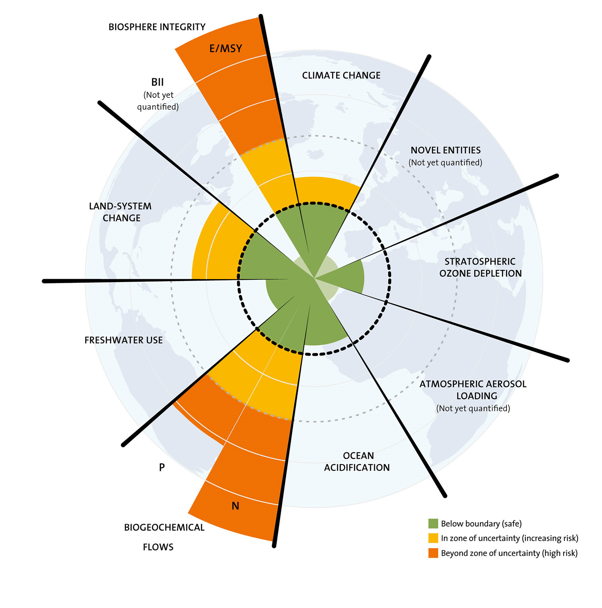
\includegraphics[width=0.5\textwidth]{sections/asset/boundy.PNG}
    \caption{Planetary boundaries. Consuming beyond Earth's bio-capacity of regeneration}
    \label{fig:badbad}
\end{figure}



%%%%%%%%%%%%%%%%%%%%%%%%%%%%%%%%%%%%%%%%
\section{Call for action}
%%%%%%%%%%%%%%%%%%%%%%%%%%%%%%%%%%%%%%%%
Extraction of natural resources surpasses the Earth's bio-capacity of regeneration and in order to maintain current consumption patters, 1.8 Earths are needed. Although, it's controversy  \parencite{Blomqvist2013, Eading1999, Rees2013, Giampietro2014} the Ecological Footprint (EF) calculation is a simple concept that gain media acceptance. International recognized organizations such as United Nations (UN) or World Wildlife Found continue to utilize the metric to indicate an illustrative estimation of the date when humans enter in a environmental deficit because the Earth's will no longer be able to regenerate. This is known as the Earth Overshot Day and from 2005 until 2018 this days were reached by the month of august. In 2018, the Earth Overshot Day was the 29th of July. \par

In 2009, the Stockholm Resilience Centre developed the Planetary Boundaries (PB) framework to define the limits within humanity can safety operate. The research identified nine systems and safety operating boundaries, where the Earth System (ES) will remain stable and consequently life on earth wont be at risk. Thanks to the scientific efforts of this research group, in 2015 it was estimated that life of Earth was already operating beyond four of those limits. \parencite{Steffen2015}.\par

Mobilized to revert the current scenario and move forward in building a global sustainable future, in 2015 world leaders agreed adopt the 2030 Agenda for Sustainable Development and the Sustainable Development Goals (SDGs). In contrast with the  Millennium Development Goals (MDGs), which mainly represents a fight against poverty, the commitment for the SDGs demands actions to be taken from all nations across the globe. A year later, the Paris Agreement was signed with the long term objective to keep global temperatures above 1.5 pre-industrial levels. This would only be achieved by cutting off emissions drastically and more efficient use of resources. \par

The Sustainable Development Goals represent an unprecedented milestone in the history of humankind. For the first time, leaders agreed to allocate resources and efforts towards 17 Goals and 169 targets. In order to move forward in global and national sustainability all countries need to make progress in all 17 Goals. Given the complexity of these systems, synergies and tensions have been identified among the SDGs and in order to make the most out of the policies, investments and efforts, resources need to be mobilized as efficiently as possible. \par

The agreement at the UN General Assembly in 2015 constituted a historical landmark in humanity. For the first time in history diverse world leaders agreed upon a general set of goals to work towards and signed the Agenda 2030 for Sustainable Development (Agenda 2030). In contrast to the Millennium Development Goals (MDGs), in this opportunity the Sustainable Development Goals (SDGs) represented a commitment that involves all countries, no matter the level of development, wealth or industrialization.  Currently 17 Goals are associated with 169 targets and a total of 232 indicators. In December of the same year, in the UN Framework Convention on Climate Change (UNFCC) the Paris Agreement (COP21) was signed to mitigate greenhouse gases (GHGs) emissions and avoid average temperature increases of 1.5C above pre-industrial levels. Both agreements show evidence of national governments and global leaders acknowledging that current practices are unsustainable and if no actions are taken to revert current trend, our support system, might become unstable and threat life on earth.\par


%%%%%%%%%%%%%%%%%%%%%%%%%%%%%%%%%%%%%%%%
\section{Cities and regions to attain the SDGs}
%%%%%%%%%%%%%%%%%%%%%%%%%%%%%%%%%%%%%%%%

Although the surface covered by cities is only cover 2\% of the earth, these areas host almost half of the global population and are responsible for 80\% of the global C02 emission, consequently; "The battle for sustainable development will be won or lost in cities" \footnote{https://www.un.org/press/en/2017/dsgsm1080.doc.htm} \footnote{https://www.undp.org/content/undp/en/home/blog/2018/battle-for-sustainable-development-will-be-won-in-cities.html} \footnote{https://www.weforum.org/agenda/2015/09/the-fight-for-sustainable-development-will-be-won-or-lost-in-our-cities/}.  \par
In 2016, the first post-Agenda2030 summit that took place was the UN Conference on Housing and Sustainable Urban Development, UN Habitat III (UNHIII), where the main objective of the Conference was to debate the details of the SDG \#11 (Make cities and human settlements inclusive, safe, resilient, and sustainable). The New Urban Agenda was the main output of UNHIII and it represents a step forward in localizing the SDGS and serves as a guide to local and regional authorities to promote sustainable practices.  \par
According to the OECD, in order to achieve at least 105 of the 169 targets local and regional engagement is required \parencite{EuropeanCommission2018, OECD2020}. Moreover, it is stressed that territorial indicators and high quality granular data are essential to move forward in the process of localizing the SDGs. Since nowadays in most countries, local governments are accountable for its citizens well-being, localizing the SDGs imply much more than implementing the SDGs, but will require active participation of local governments in defining the policies needed to achieve the SDGs targets. \par
In the light of the year 2020 events, it has become clear that much urban and regional research is needed to understand city dynamics, how they interact with other urban settlements and resource hubs. Definitely, cities (and the network of them) will play a crucial role in achieving the SDGs and planning tools are needed to ensure enhance resiliency against diverse threats.   



\section{On the importance of Circular Economy}
According  the Circularity Report gap \parencite{CircleEconomy2020}, "Today, the global economy is only 8.6\% circular — just two years ago it was 9.1\%. There are reasons for this negative trend, but the result remains the same: the news is not just bad, it is worse. This negative trend can be explained by three key related, underlying trends: high rates of extraction; ongoing stock build- up; and, increasing (but still low) levels of end-of- use processing and cycling. These underlying trends are deeply embedded within the ‘take-make-waste’ tradition of the linear economy — the problems are hardwired. As such, the outlook for closing the circularity gap looks bleak under the dead hand of business as usual. We desperately need transformative and correctional solutions; change is a must."\par
Implementing CE strategies can be used to successfully meet several of the SDGs. Direct positive effects are associated with SDGs 7, 8, 12, 6 and 15 \parencite{Schroeder2018}. 

\begin{figure}[h!]
    \centering
    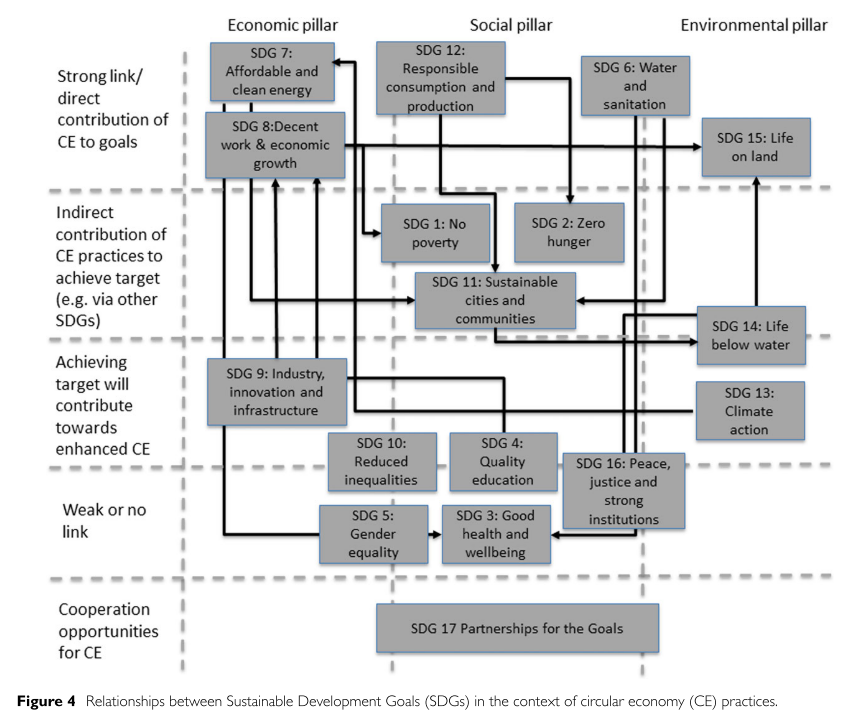
\includegraphics[width=0.7\textwidth]{sections/asset/ce_relation.PNG}
    \caption{Circular economy contributions to SDG}
    \label{fig:badbad}
\end{figure}


According to a study conducted by the Ellen MacArthur Foundation and McKinsey in 2015, adopting a circular economy approach could boost the continent’s resource productivity by 3\% by 2030, generate cost savings of 600 billion Euros a year and bring 1.2 trillion Euros in other non-resource and externality benefits. The key areas of benefit are mobility, food and buildings. Another 2015 study by the United Kingdom’s Waste and Resources Action Programme found that a circular economy has the potential to create 1.2 to 3 million jobs in Europe by 2030. \par


Ellen McArthur Foundation defines CE as a \cite{systemic approach to economic development designed to benefit businesses, society, and the environment. In contrast to the ‘take-make-waste’ linear model, a circular economy is regenerative by design and aims to gradually decouple growth from the consumption of finite resources. After defining what an economy actually is, this learning path explores the nuances of the concept of a circular economy, including the difference between biological and technical materials, the different opportunities that exist to keep materials and products in use, and the history of the idea.} \par
Still, under the view of certain academics the concept is still evolving and since is still in early stages of development, much research is needed to explore its meaning, applications and implications \parencite{Ghisellini2016}. According to \textcite{Kirchherr2017} the main aim of the CE is considered to be economic prosperity, followed by environmental quality; social equity and future generations is barely mentioned. \par

\begin{figure}[h!]
    \centering
    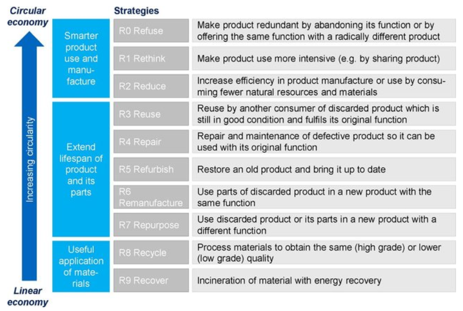
\includegraphics[width=0.7\textwidth]{sections/asset/rs.png}
    \caption{Circular economy vs linear economy strategies}
    \label{fig:badbad}
\end{figure}


The concept of CE has been introduced to cities and some authors have trying to translate what does this means for urban and regional planning \parencite{Williams2019}. 

\begin{figure}[h!]
    \centering
    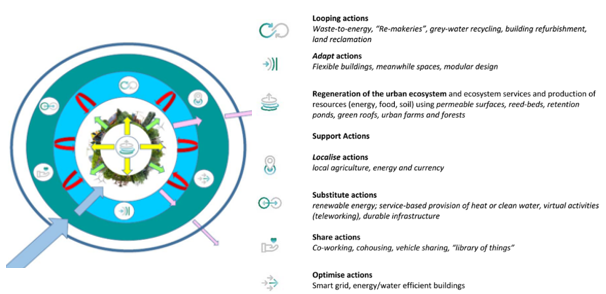
\includegraphics[width=0.7\textwidth]{sections/asset/city.PNG}
    \caption{Circular economy conceptualization for cities}
    \label{fig:badbad}
\end{figure}
